%!TEX root = ./main.tex

\section{Resugaring by Lazy Desugaring}
\label{sec3}

In this section, we present our new approach to resugaring. Different from the traditional approach that clearly separates the surface and the core languages, we combine them together as one mixed language, allowing users to freely use the language constructs in both languages. We will show that any expression in the mixed language can be evaluated in such a smart way that a sequence of all expressions that are necessarily to be resugared by the traditional approach can be correctly produced.

\subsection{Mixed Language for Resugaring}

\begin{figure}[t]
	\[
	\begin{array}{lllll}
	 &\m{CoreExp} &::=& x  & \note{variable}\\
	       &&~|~& c  & \note{constant}\\
				 &&~|~& (\m{CoreHead}~\m{CoreExp}_1~\ldots~\m{CoreExp}_n) & \note{constructor}\\
	\\
	 &\m{SurfExp} &::=& x  & \note{variable}\\
	       &&~|~& c  & \note{constant}\\
				 &&~|~& (\m{CoreHead}~\m{SurfExp}_1~\ldots~\m{SurfExp}_n) & \note{selected core constructor}\\
					 &&~|~& (\m{SurfHead}~\m{SurfExp}_1~\ldots~\m{SurfExp}_n) & \note{sugar expression}\\
	\end{array}
	\]
	\caption{Core and Surface Expressions}
	\label{fig:expression}
\end{figure}

We will define a mixed language for a given core language and a surface language defined over the core language. An expression in this language will be reduced step by step by the reduction rules for the core language and the desugaring rules for defining the syntactic sugars in the surface language.

\subsubsection{Core Language}

For our host language, we consider its evaluator as a blackbox \todo{need to be corrected.} but with two natural assumptions. First, there is a deterministic stepper in the evaluator which, given an expression in the host language, can deterministically reduce the expression to a new expression. Second, the evaluation of any sub-expression has no side-effect on other parts of the whole expression.

An expression of the core language is defined in Figure \ref{fig:expression}. It is a variable, a constant, or a (language) constructor expression. Here, $\m{CoreHead}$ stands for a language constructor such as $\m{if}$ and $\m{let}$. To be concrete, we will use the core language defined in Figure \ref{fig:core} to demonstrate our approach.

\begin{figure}[t]
\begin{center}
\begin{tabularx}{.96\textwidth}%
{|>{\setlength{\hsize}{.5\hsize}\centering\arraybackslash}X  |>{\setlength{\hsize}{1.5\hsize}\centering\arraybackslash}X|}
%{|*{2}{>{\centering\arraybackslash}X|}}
\hline
Syntax & Reduction rules \\ \hline
(if e e e) &\qquad\qquad\qquad(if \#t e2 e3) $\dashrightarrow$ e2 \newline ~(if \#f e2 e3) $\dashrightarrow$ e3\\ \hline
((lam (x ...) e) e ...) & ((lam (x0 x1 ...) e) v0 v1 ...) $\dashrightarrow$ (let ((x0 v0) ((lam (x1 ...) e) v1 ...))\\ \hline
((lamN (x ...) e) e ...) & ((lamN (x0 x1 ...) e) e0 e1 ...) $\dashrightarrow$ (let ((x0 e0) ((lamN (x1 ...) e) e1 ...))\\ \hline
(let ((x e) ...) e) & (let ((x0 e0) (x1 e1) ...) e) $\dashrightarrow$ (let ((x1 e1) ...) (subst x0 e0 e))\newline (let () e)  $\dashrightarrow$ e (where subst is a meta function)\\ \hline
(first e) & (first (list v1 v2 ...)) $\dashrightarrow$ v1\\ \hline
(rest e) & (rest (list v1 v2 ...)) $\dashrightarrow$ (list v2 ...)\\ \hline
(empty e) & \qquad\qquad\qquad(empty (list)) $\dashrightarrow$ \#t \newline (empty (list v1 ...)) $\dashrightarrow$ \#f\\ \hline
(cons e e) & (cons v1 (list v2 ...)) $\dashrightarrow$ (list v1 v2 ...)\\ \hline
(op e e) \newline op=+-*/><== & (op v1 v2) $\dashrightarrow$ arithmetic result\\ \hline
\end{tabularx}
\end{center}
\caption{An Core Language Example}
\label{fig:core}
\end{figure}


%For simplicity, we use the prefix notation. For instance, we write $\m{if-then-else}~e_1~e_2~e_3$, which would be more readable if we write $\m{if}~e_1~\m{then}~e_2~\m{else}~e_3$. In this paper, we may write both if it is clear from the context.

\subsubsection{Surface Language}

Our surface language is defined by a set of syntactic sugars, together with some language constructs in the core language. So an expression of the surface language is some core constructor expressions with sugar expressions, as defined in Figure \ref{fig:expression}.

A syntactic sugar is defined by a desugaring rule in the following form:
\[
\drule{(\m{SurfHead}~x_1~x_2~\ldots~x_n)}{\m{Exp}}
\]
where its LHS is a simple pattern (unnested) and its RHS is a surface expression. For instance, we may define syntactic sugar \m{And} by
\[
\drule{(\m{And}~x~y)}{(\m{if}~x~y~\false)}.
\]
Note that if the pattern is nested, we can introduce a new syntactic sugar to flatten it.
One may wonder why not restricting the RHS to be a core expression $\m{CoreExp}$, which sounds more natural. We use $\m{surfExp}$ to be able to allow definition of recursive syntactic sugars, as seen in the following example.
\[
\begin{array}{l}
\drule{(\m{Odd}~x)}{\m{if}~(>~x~0)~(\m{Even}~(−~x~1))~\false)}\\
\drule{(\m{Odd}~x)}{\m{if}~(>~x~0)~(\m{Odd}~(−~x~1))~\true)}
\end{array}
\]

We assume that all desugaring rules are not overlapped in the sense that for a syntactic sugar expression, only one desugaring rule is applicable.


\subsubsection{Mixed Language}

\begin{figure}[t]
\begin{centering}
	\framebox[36em][c]{
		\parbox[t]{33em}{
			\[
			\begin{array}{lcl}
			\m{Exp} &::=& \m{DisplayableExp}\\
			&|& \m{UndisplayableExp}\\
\\
			\m{DisplayableExp} &::=& \m{SurfExp}\\
			&|& \m{CommonExp}
\\
			\m{UndisplayableExp} &::=& \m{Core'Exp}\\
			&|& \m{OtherSurfExp}\\
			&|& \m{OtherCommonExp}\\
\\
			\m{CoreHead} &::=& \m{CoreHead'}\\
						 &|& \m{CommonHead}\\
\\						
			\m{Core'Exp} &::=& (\m{CoreHead'}~\m{Exp}*)\\
\\
			\m{SurfExp} &::=& (\m{SurfHead}~\m{DisplayableExp}*)\\
\\
			\m{CommonExp} &::=& (\m{CommonHead}~\m{DisplayableExp}*)\\
			&|& c \qquad \note{// constant value}\\
			&|& x \qquad \note{// variable} \\
\\
			\m{OtherSurfExp} &::=& (\m{SurfHead}~\m{Exp}*~\m{UndisplayableExp}~\m{Exp}*)\\
\\
			\m{OtherCommonExp} &::=& (\m{CommonHead}~\m{Exp}*~\m{UndisplayableExp}~\m{Exp}*)
			\end{array}
			\]
		}
	}
\end{centering}
\caption{Our Mixed Language}
\label{fig:mix}
\end{figure}

Our mixed language for resugaring combines the surface language and the core language.
%
The difference between our core language (CoreLang) and our surface language (SurfLang) is identified by their \m{Head}. But there are some terms in the core language should be displayed during evaluation, or we need some terms to help us getting better resugaring sequences. So we defined \m{CommonExp}, which origin from CoreLang, but can be displayed in resugaring sequences. The \m{Core'Exp} terms are terms with undisplayable \m{CoreHead} (named \m{CoreHead'}. The \m{SurfExp} terms are terms with \m{SurfHead} and all sub-expressions are displayable. The \m{CommonExp} terms are terms with displayable CoreLang's \m{Head} (named \m{CommonHead}, together with displayable sub-expressions. There exists some other expression during our resugaring process, which have displayable \m{Head}, but one or more subexpressions cannot. They are \m{UndisplayableExp}.

Take some terms in the core language in Figure \ref{fig:core} as examples.
We may assume \m{if}, \m{let}, \m{$\lambda _{N}$} (call-by-name lambda calculus), \m{empty}, \m{first}, \m{rest} as \m{CoreHead'}, \m{op}, \m{$\lambda$}, \m{cons} as \m{CommonHead}. Then we would show some useful intermediate steps.

Note that some expressions with \m{CoreHead} contains subexpressions with \m{SurfHead}, they are of \m{CoreExp} but not in core language, we need a tricky extension for the core language's evaluator. For expression \Code{(CoreHead $e_1$ ... $e_n$)}, replacing all subexpression not in core language with different reduciable core language's term. Then getting a result after inputting the new expression \Code{exp'} to the original blackbox stepper. If reduction appears at subexpressions after \Code{$e_i$} replaced by, then the stepper with the extension should return \Code{(CoreHead $e_1$ ... $e_i'$ ... $e_n$)}, where $e_i'$ is $e_i$ after desugaring. (an  example in Fig \ref{fig:e1}) Otherwise, stepper should return \Code{exp'}, with all the replaced subexpressions replacing back. (an example in Fig \ref{fig:e2}) The extension will not vialate properties of original core language's evaluator. It is obvious that the evaluator with the extension will reduce at the subexpression as it needs in core language, if the reduction appears in s subexpression.

\begin{center}
\begin{figure}[h]
\centering
\Code{(if (and e1 e2) true false)}\\ $\Downarrow_{replace}$\\ \Code{(if tmpe1 true false)}\\ $\Downarrow_{blackbox}$\\ \Code{(if tmpe1' true false)}\\ $\Downarrow_{desugar}$\\ \Code{(if (if e1 e2 false))}
\caption{e1}
\label{fig:e1}
\end{figure}

\begin{figure}[h]
\centering
\Code{(if (if true ture false) (and ...) (or ...))}\\ $\Downarrow_{replace}$ \\\Code{ (if (if true ture false) tmpe2 tmpe3)}\\ $\Downarrow_{blackbox}$\\  \Code{(if true tmpe2 tmpe3)}\\ $\Downarrow_{reback}$\\ \Code{(if true (and ...) (or ...))}
\caption{e2}
\label{fig:e2}
\end{figure}


 % \Code{(if true (and ...) (or ...))} $\Rightarrow_{replace}$ \Code{(if true tmpe2 tmpe3)} $\Rightarrow_{blackbox}$ \\ \Code{tmpe2} $\Rightarrow_{replaceback}$ \Code{(and ...)}

\end{center}

\subsection{Resugaring Algorithm}

Our resugaring algorithm works on our mixed language, based on the reduction rules of the core language and the desugaring rules for defining the surface language. Let $\redc{}{}$ denote the one-step reduction of the core language (based on the blackbox stepper with extension, and $\drule{}{}$ the one-step desugaring of outermost sugar. We define $\redm{}{}$, the one-step reduction of our mixed language, as follows.

\infrule[CoreRed]
{\redc{(\m{CoreHead}~e_1~\ldots~e_n)}{e'}}
{\redm{(\m{CoreHead}~e_1~\ldots~e_n)}{e'}}

\infrule[SurfRed1]
{\drule{(\m{SurfHead}~x_1~\ldots~x_i~\ldots~x_n)}{e},~\redm{e_i}{e_i''}\\
\exists i.\, \redm{e[e_1/x,\ldots,e_i/x_i,\ldots,e_n/x_n]}{e[e_1/x,\ldots,e_i'/x_i,\ldots,e_n/x_n]}
}
{\redm{(\m{SurfHead}~e_1~\ldots~e_i~\ldots~e_n)}{(\m{SurfHead}~e_1~\ldots~e_i''~\ldots~e_n)}}

\infrule[SurfRed2]
{\drule{(\m{SurfHead}~x_1~\ldots~x_i~\ldots~x_n)}{e}\\
\neg \exists i.\, \redm{e[e_1/x_1,\ldots,e_i/x_i,\ldots,e_n/x_n]}{e[e_1/x_1,\ldots,e_i'/x_i,\ldots,e_n/x_n]}
}
{\redm{(\m{SurfHead}~e_1~\ldots~e_i~\ldots~e_n)}{e[e_1/x_1,\ldots,e_i/x_i,\ldots,e_n/x_n]}
}

The \m{CoreRed} rule describes how our mixed language handle expressions with \m{CoreHead}---just leave it to the core language's evaluator. Then for the expression with \m{SurfHead}, we will firstly desugar the outermost sugar (identified by the \m{SurfHead}), then recursively executing $\redm{}{}$. In the recursive call, if one of original subexpression $e_i$ is reduced (\m{SurfRed1}), then the original sugar is not necessarily desugared, we should only reduce the subexpression $e_i$; if not (\m{SurfRed2}), then the sugar have to desugar.

%\todo{Add explanantion of the above rule.}

Then our desugaring algorithm is defined based on $\redm{}{}$.

\[
\begin{array}{llll}
\m{desugar} (e) &=& \key{if}~\m{isNormal}(e)~\key{then}~return\\
              & & \key{else}~\\
							& & \qquad \key{let}~\redm{e}{e'}~\key{in}\\
							& & \qquad \key{if}~e' \in~\m{DisplayableExp} \\
							& & \qquad \qquad \m{output}(e'),~\m{desugar}(e')\\
							& & \qquad \key{else}~\m{desugar}(e')
\end{array}
\]

We use the \m{DisplayableExp} to restrict immediate sequences to be output or not. It is more explicit compared to existing approaches.

\subsection{Correctness}

First of all, because the difference between our lightweight resugaring algorithm and the existing one is that we only desugar the syntactic sugar when needed, and in the existing approach, all syntactic sugar desugars firstly and then executes on CoreLang.

Then, to prove convenience, define some terms.

$Exp~=~(Headid\;Subexp_{1}\;Subexp_{\ldots} \ldots)$ is any reducible expression in our language.

If we use the reduction rule that desugar Exp's outermost syntactic sugar, then the reduction process is called {\bfseries Outer Reduction}.

If the reduction rule we use reduce $Subexp_{i}$, where $Subexp_{i}$ is $(Headid_{i}~Subexp_{i1}~Subexp_{i\ldots} \ldots)$
\begin{itemize}
	\item If the reduction process is Outer Reduction of $Subexp_{i}$ = $(Headid_{i}~Subexp_{i1}~Subexp_{i\ldots} \ldots)$, then it is called {\bfseries Surface Reduction}.
	\item If the reduction process reduces $Subexp_{ij}$, then it is called {\bfseries Inner Reduction}.
\end{itemize}

{\bfseries Example:}

$(\mbox{if}\; \#t\; Exp_{1}\; Exp_{2})$ → $Exp1$ \hfill Outer Reduction

$(\mbox{if}\; (\mbox{And}\; \#t\; \#f)\; Exp_{1}\; Exp_{2})$ → $(\mbox{if}\; (\mbox{if}\; \#t\; \#f\; \#f)\; Exp_{1}\; Exp_{2})$ \hfill Surface Reduction

$(\mbox{if}\; (\mbox{And}\; (\mbox{And}\; \#t\; \#t)\; \#t) \; Exp_{1}\; Exp_{2})$ → $(\mbox{if}\; (\mbox{And}\; \#t\; \#t)\; Exp_{1}\; Exp_{2})$ \hfill Inner Reduction

\begin{Def}[Upper and lower expression]
For $Exp$=$(Headid\;Subexp_{1}\;Subexp_{\ldots} \ldots)$, $Exp$ is called {\bfseries upper expression}$,Subexp_{i}$is called {\bfseries lower expression}.
\end{Def}

Case 2, 4, 6 in the core algorithm are of outer reduction. And case 3 or 5 are of surface reduction if the reduced subexpression is processed by outer reduction, or they are of inner reduction.
What we need to prove is that all the 6 cases of core algorithm core-algo satisfy the properties. Case 1 and case 2 won't effect any properties, because it does what CoreLang should do.

\begin{Def}[Emulation]

For~\m{Exp}=$(\m{SurfHead}~e_1~\ldots~e_i~\ldots~e_n)$,\\ if~$\redm{\m{Exp}}{\m{Exp'}}$ and \m{Desugar}(\m{Exp})$\not=$$\m{Desugar}(\m{Exp'})$,~then $\redc{\m{Desugar}(\m{Exp})}{\m{Desugar}(Exp')}$
\end{Def}

\begin{lemma}

For~\m{Exp}=$(\m{SurfHead}~e_1~\ldots~e_i~\ldots~e_n)$,\\ if inputting $\m{Desugar}(\m{Exp})$ to core language's evaluator reduces the term original from $e_i$ in one step, then the $\redm{}{}$ will reduce \m{Exp} at $e_i$.

%then $\redc{\m{Desugar}(\m{Exp})}{\m{Desugar}(\m{Exp'})}$
\end{lemma}

\begin{proof}
For $\drule{(\m{SurfHead}~x_1~\ldots~x_i~\ldots~x_n)}{e}$

if $e$ is of normal form, the $\m{Desugar}(\m{Exp})$ will not be reduced by core evaluator.

if $e$ is headed with \m{CoreHead}, then according to the \m{CoreRed} rule, the $\redc{}{}$ will execute on $e$, which will reduce the subexpression $e_i$ according to the blackbox evaluator with extension. Then the \m{SurfRed2} rule will reduce $e_i$. Because of the extension of evaluator reduces the subexpression in correct location, so it is for $\redm{}{}$.

if $e$ is headed with \m{SurfHead}, then the $redm{}{}$ will execute recursively on $e$. If the new one satisfies the lemma, then it is for the former. Because any sugar expression will finally be able to desugar to expression with \m{CoreHead}, it can be proved recursively.
\end{proof}
\begin{proof}[Proof of Emulation]
\hfill

For \m{SurfRed1} rule, $\redm{(\m{SurfHead}~e_1~\ldots~e_i~\ldots~e_n)}{(\m{SurfHead}~e_1~\ldots~e_i''~\ldots~e_n)}$, where $\redm{e_i}{e_i''}$. 
If $\m{Desugar}(e_i)$=$\m{Desugar}(e_i'')$, then \m{Desugar}(\m{Exp})=\m{Desugar}(\m{Exp'}). If not,  what we need to prove is that, $\redc{\m{Desugar}(\m{Exp})}{\m{Desugar}(\m{Exp'})}$. Note that the only difference between \m{Exp} and \m{Exp'} is the i-th subexpression, and we have proved the lemma that the subexpression is the one to be reduced after the expression desugared totally, it will be also a recursive proof on the subexpression $e_i$.

For \m{SurfRed2} rule, \m{Exp'} is \m{Exp} after the outermost sugar resugared. So \m{Desugar}(\m{Exp})=\m{Desugar}(\m{Exp'}).

\end{proof}

\begin{proof}[Proof of Abstraction]
\hfill\\
It's true, because we only display the sequence which satisfies abstraction property.
\end{proof}

\begin{lemma}
If no syntactic sugar desugared before necessary (if the sugar not desugared, the expression of mixed language cannot be reduced after other sugars desugared, then coverage property is satisfied.
\end{lemma}

\begin{proof}[Proof of Lemma3.2]
Assume that no syntactic sugar not necessarily expanded desugars too early, existing an expression in CoreLang

$Exp$ = $(\m{Head}~e_1~\ldots~e_i~\ldots~e_n)$ which can be resugared to

$ResugarExp'$ = $(Surfid\;Subexp'_{1}\;Subexp'_{\ldots}\ldots)$, and $ResugarExp'$ is not displayed during lightweight-resugaring process. Then

\begin{itemize}
	\item Or existing

	$ResugarExp$=$(Surfid\;Subexp'_{1}\;\ldots\;Subexp_{i}\;Subexp'_{\ldots}\ldots)$ in resugaring sequences, such that the expression after $ResugarExp$ desugaring reduces to $Exp$, and the reduction reduces $ResugarExp$'s sub-expression $Subexp_{i}$. If so, outermost syntactic sugar of $ResugarExp$ is not expanded. So if $ResugarExp'$ is not displayed, then the sugar not necessarily expanded desugars too early, which is contrary to assumption.


	\item Or existing

	$ResugarExp$=$(Surfid'\;\ldots\;ResugarExp'\;\ldots)$ in resugaring sequences, such that the expression after $ResugarExp$ desugaring reduces to $Exp$, and $Exp$ is desugared from $ResugarExp'$'s sub-expression. If $ResugarExp'$ is not displayed, then the outermost syntactic sugar is expanded early, which is contrary to assumption.
	\item Or though the $Exp$ exists, it doesn't from $ResugarExp$.

\end{itemize}
\end{proof}

\begin{proof}[Proof of Coverage]
\hfill\\
For case 4 and 6, the syntactic sugar has to desugar.

For case 3 and 5, the reduction occurs in sub-expression of $Exp$. So if applying core algorithm core-algo on the subexpression doesn't desugar syntactic sugars not necessarily expanded, then this two cases don't. If the reduction is surface reduction, then the reduction of the subexpression is processed by case 2, 4 or 6, which don't desugar sugars not necessarily expanded; if the reduction is inner reduction, then it's another recursive proof as emulation. So in these two cases, the core-algo only desugar the sugar which has to be desugared.
\end{proof}

\subsection{Implementation}

Our lightweight resugaring approach  is implemented using PLT Redex\cite{SEwPR}, which is an semantic engineering tool based on reduction semantics\cite{reduction}. The whole framework is as Fig\ref{fig:frame}.

\begin{figure}[h]
	\centering
	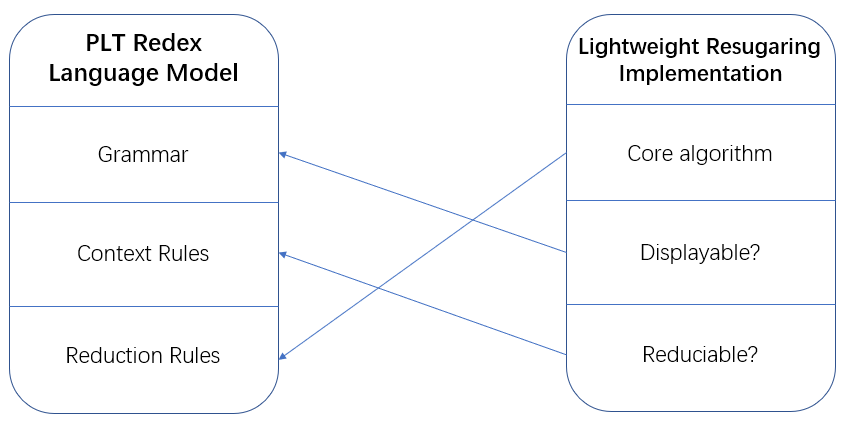
\includegraphics[width=12cm]{images/frame.png}
	\caption{framework of implementation}
	\label{fig:frame}
\end{figure}

The grammar of the whole language contains Coreexp', Surfexp and Commonexp as the language setting in sec\ref{sec3}. OtherSurfexp is of Surfexp and OtherCommonexp is of Commonexp. The identifier of any kind of expression is Headid of expression. If we need to add a syntactic sugar to the whole language, only three steps is needed.

\begin{enumerate}
\item Add grammar of the syntactic sugar.
\item Add context rules of the sugar, such that any sub-expressions can be reduced.
\item Add desugar rules of the sugar to reduction rules of the whole language.
\end{enumerate}

Then inputting an expression of the syntactic sugar to lightweight-resugaring will get the resugaring sequences.

\subsection{Application}

We test some applications on the tool implemented using PLT Redex. Note that we set CBV's lambda calculus as terms in commonexp, because we need to output some intermediate sequences including lambda expressions in some examples. It's easy if we want to skip them.

\subsubsection{simple sugar}
\label{mark:simple}

We construct some simple syntactic sugar and try it on our tool. Some sugar is inspired by the first work of resugaring\cite{resugaring}. The result shows that our approach can handle all sugar features of their first work.

We take a SKI combinator syntactic sugar as an example. We will show why our approach is lightweight.
\begin{Codes}
	S \DeStep{ (lamN (x1 x2 x3) (x1 x2 (x1 x3)))}
	K \DeStep{ (lamN (x1 x2) x1)}
	I \DeStep{ (lamN (x) x)}
\end{Codes}



Although SKI combinator calculus is a reduced version of lambda calculus, we can construct combinators' sugar based on call-by-need lambda calculus in our CoreLang. For expression

 $(S~(K~(S~I))~K~xx~yy)$, we get the following resugaring sequences as following.
\begin{Codes}
    (S (K (S I)) K xx yy)
\OneStep (((K (S I)) xx (K xx)) yy)
\OneStep (((S I) (K xx)) yy)
\OneStep (I yy ((K xx) yy))
\OneStep (yy ((K xx) yy))
\OneStep (yy xx)
\end{Codes}


For existing approach, the sugar expression should firstly desugar to
\begin{Codes}
((lamN
   (x_{1} x_{2} x_{3})
   (x_{1} x_{3} (x_{2} x_{3})))
  ((lamN (x_{1} x_{2}) x_{1})
   ((lamN
     (x_{1} x_{2} x_{3})
     (x_{1} x_{3} (x_{2} x_{3})))
    (lamN (x) x)))
  (lamN (x_{1} x_{2}) x_{1})
  xx yy)
\end{Codes}

Then in our CoreLang, the execution of expanded expression will contain 33 steps. For each step, there will be many attempts to match and substitute the syntactic sugars. It will omit more steps for a larger expression.

So the unidirectional resugaring algorithm makes our approach lightweight, because no attempts for resugaring the expression take place.
\subsubsection{hygienic macro}
\label{mark:hygienic}


The second work\cite{hygienic} mainly processes hygienic macro compared to first work. It use a DAG to represent the expression. However, hygiene is not hard to handle by our lazy desugaring strategy. Our algorithm can easily process hygienic macro without special data structure. 
% The $Let$ sugar is define as follow
% \begin{Codes}
% 	(Let x e exp) \DeStep{ ((lambda (x) exp) e)}
% \end{Codes}
% % $(Let\;x\;v\;exp)$ $\rightarrow$ $(Apply\;(\lambda\;(x)\;exp)\;v)$

% Take $(Let~x~1~(+~x~(Let~x~2~(+~x~1))))$ for an example. First, a temp expression

% $(Apply\;(\lambda\;(x)\;(+~x~(Let~x~2~(+~x~1))))\;1)$

% is needed. (case 5 or 6)Then one-step try on the temp expression, we will get

% $(+~1~(Let~1~2~(+~1~1)))$ which is out of the whole language's grammar. In this case, it is not a good choice to desugar the outermost $Let$ sugar. Then we just apply the core-algo on the sub-expression where the error occurs ($(+~x~(Let~x~2~(+~x~1)))$ in this example). So the right intermediate sequence $(Let~x~1~(+~x~3))$ will be get.

A typical hygienic example is as the example origined from Hygienic resugaring\cite{hygienic}. We simplify the example to the following one. 
\begin{Codes}
	(Hygienicadd e1 e2) \DeStep{ (let ((x e1)) (+ x e2))}
\end{Codes}

For existing resugaring approach, if we want to get sequences of \Code{(let ((x 2)) (Hygienicadd 1 x))}, it will firstly desugar to \Code{(let ((x 2)) (let ((x 1)) (+ x x)))}, but it is awful because the two $x$ in \Code{(+ x x)} should be bind to different value. But for our lazy desugaring, the \m{hygienicadd} sugar does not have to desugar until necessary, so, getting following sequences.

\begin{Codes}
    (let ((x 2)) (Hygienicadd 1 x)
\OneStep{ (Hygienicadd 1 2)}
\OneStep{ (+ 1 2)}
\OneStep{ 3}
\end{Codes}

The lazy desugaring is also comvinent for hygienic resugaring for non-hygienic core language. For example, \Code{(let ((x 1)) (+ x (let ((x 2)) (+ x 1))))} may be reduced to \Code{(+ 1 (let ((1 2)) (+ 1 1)))} by a simple core language whose \Code{let} expression does not handle cases like that. But by writing a simple sugar Let,
\[\drule{(Let~e_1~e_2~e_3)}{(let~((e_1~e_2))~e_3)}\]
and some simple modifies in the reduction of mixed language, we will get the following sequences in our system.
\begin{Codes}
    (Let x 1 (+ x (Let x 2 (+ x 1))))
\OneStep{(Let x 1 (+ x (+ 2 1)))}
\OneStep{(Let x 1 (+ x 3))}
\OneStep{(+ 1 3)}
\OneStep{4}
\end{Codes}

In practical application, we think hygiene can be easily processed by rewriting system. But our result shows lazy desugaring is really a good way to handle hygienic macro in any systems.

\subsubsection{recursive sugar}
Recursive sugar is a kind of syntactic sugars where call itself or each other during the expanding. For example,

\begin{Codes}
(Odd e) \DeStep{ (if (> e 0) (Even (- e 1)) \#f)}
(Even e) \DeStep{ (if (> e 0) (Odd (- e 1)) \#t)}
\end{Codes}
are typical recursive sugars. The existing resugaring approach can't process this kind of syntactic sugar easily, because boundary conditions are in the sugar itself.

Take $(Odd~2)$ as an example. The previous work will firstly desugar the expression using the rewriting system. Then the rewriting system will never terminate as following shows.
\begin{Codes}
   (Odd 2)
\DeStep{ (if (> 2 0) (Even (- 2 1) \#f))}
\DeStep{ (if (> (- 2 1) 0) (Odd (- (- 2 1) 1) \#t))}
\DeStep{ (if (> (- (- 2 1) 1) 0) (Even (- (- (- 2 1) 1) 1) \#f))}
\DeStep{ ...}
\end{Codes}


Then the advantage of our approach is embodied. Our lightweight approach doesn't require a whole expanding of sugar expression, which gives the framework chances to judge boundary conditions in sugars themselves, and showing more intermediate sequences. We get the resugaring sequences of the former example using our tool.
\begin{Codes}
    (Odd 2)
\OneStep{ (Even (- 2 1))}
\OneStep{ (Even 1)}
\OneStep{ (Odd (- 1 1))}
\OneStep{ (Odd 0)}
\OneStep{ \#f}
\end{Codes}


We also construct some higher-order syntactic sugars and test them. The higher-order feature is important for constructing practical syntactic sugar. And many higher-order sugars should be constructed by recursive defination. The first sugar is \m{filter}, implemented by pattern matching term rewriting.

\begin{Codes}
   (filter e (list v1 v2 ...))
\DeStep{ (if (e v1) (cons v1 (filter e (list v2 ...)))\ (filter e (list v2 ...)))}
   (filter e (list)) \DeStep{ (list)}
\end{Codes}
and getting the following result. (by making \Code{(lam ...)} \m{CommonExp} )

\begin{Codes}
    (filter (lam (x) (and (> x 1) (< x 4))) (list 1 2 3 4))
\OneStep{ (filter (lam (x) (and (> x 1) (< x 4))) (list 2 3 4))}
\OneStep{ (cons 2 (filter (lam (x) (and (> x 1) (< x 4))) (list 3 4)))}
\OneStep{ (cons 2 (cons 3 (filter (lam (x) (and (> x 1) (< x 4))) (list 4))))}
\OneStep{ (cons 2 (cons 3 (filter (lam (x) (and (> x 1) (< x 4))) (list))))}
\OneStep{ (cons 2 (cons 3 (list)))}
\OneStep{ (cons 2 (list 3))}
\OneStep{ (list 2 3)}
\end{Codes}

Here, although the sugar can be processed by existing resugaring approach, it will be rebundant. The reason is that, a filter for a list of length $n$ will match to find possible resugaring $n*(n-1)/2$ times. Thus, lazy desugaring is really important to reduce the resugaring complexity of recursive sugar.

Moreover, just like the \emph{Odd and Even} sugar above, there are some simple rewriting systems which do not allow pattern-based rewriting. Or there are some sugars which need to be expressed by the terms in core language as conditions. Take the example of another higher-order sugar \m{map} as an example.
\begin{Codes}
    (map e1 e2)
\DeStep{ (let ((x e2)) (if (empty? x) (list) (cons (e_1 (first x)) (map e_1 (rest x)))))}
\end{Codes}
Get following resugaring sequences.
\begin{Codes}
    (map (lam (x) (+ x 1)) (cons 1 (list 2)))
\OneStep{ (map (lam (x) (+ x 1)) (list 1 2))}
\OneStep{ (cons 2 (map (lam (x) (+ 1 x)) (list 2)))}
\OneStep{ (cons 2 (cons 3 (map (lam (x) (+ 1 x)) (list))))}
\OneStep{ (cons 2 (cons 3 (list)))}
\OneStep{ (cons 2 (list 3))}
\OneStep{ (list 2 3)}
\end{Codes}

Note that the \m{let} term is to limit the subexpression only appears once in RHS. In this example, we can find that the list \Code{(cons 1 (list 2))}, though equal to \Code{(list 1 2)}, is represented by core language's term. So it will be difficult to handle the inline boundary conditions by rewriting system. But our approach is easy to handle cases like this.

\subsection{Compare to previous work}

As mentioned many times before, the biggest difference between previous resugaring approach and our approach, is that our approach doesn't need to desugar the sugar expresssion totally. Thus, our approach has the following advantages compared to previous work.

\begin{itemize}
	\item {\emph Lightweight} As the example at sec\ref{mark:simple}, the match and substitution process searchs all intermediate sequences many times. It will cause huge cost for a large program. So out approach---only expanding a syntactic sugar when necessarily, is a lightweight approach.
	\item {\emph Friendly to hygienic macro} Previous hygienic resugaring approach use a new data structure---abstract syntax DAG, to process resugaring of hygienic macros. Our approach simply finds hygienic error after expansion, and gets the correct reduction instead.
	\item {\emph More syntactic sugar features} The ability of processing non-pattern-based (\todo{inline?}) recursive sugar is a superiority compared to previous work. The key point is that recursive syntactic sugar must handle boundary conditions. Our approach handle them easily by not necessarily desugaring all syntactic sugars. Higher-order functions, as an important feature of functional programming, was supported by many daily programming languages. Lazy desugaring makes writing higher-order sugars easier.
	% \item {\emph Rewriting rules based on reduction semantics} Any syntactic sugar that can expressed by reduction semantics can be used in our approach. It will give more possible forms for constructing syntactic sugars. todo:example?
\end{itemize}

% The most obvious shortage compared to existing approach is that our approach needs a whole semantic of core languages. The reason is because in case 5 and 6, we need to expand the outermost syntactic sugar and try one step, which may contain unexpanded sugars. Theoretically, our dynamic approach would also work with only a core language's stepper, by totally expand all sugar expressions and marked where each term is originated from. Simple modifications are needed in core-algo. But we did not try it, because of the intent we would discussed in Sec\ref{mark:assumption}.
